\documentclass[11pt]{article}

\usepackage[T1]{fontenc}
\usepackage[utf8]{inputenc}
\usepackage[english]{babel}
\usepackage{mathpazo}
\usepackage[scaled]{helvet}
\usepackage{microtype}
\usepackage[letterpaper,margin=0.88in]{geometry}
\usepackage{amsmath}
\usepackage{amssymb}
\usepackage{booktabs}
\usepackage{array}
\usepackage{tabularx}
\usepackage{enumitem}
\usepackage{xcolor}
\usepackage{float}
\usepackage{graphicx}
\usepackage{listings}
\usepackage{tikz}
\usetikzlibrary{arrows.meta,positioning}
\usepackage{xurl}
\usepackage{hyperref}

\hypersetup{
  pdftitle={Jörmungandr: A Plugin Runtime for Distributed Reinforcement Learning},
  pdfauthor={research@strategynet.ai},
  colorlinks=true,
  linkcolor=blue!50!black,
  citecolor=blue!50!black,
  urlcolor=blue!60!black
}

\setlength{\parindent}{0pt}
\setlength{\parskip}{0.52em}
\setlist{nosep}

\lstdefinestyle{jorm}{
  basicstyle=\ttfamily\footnotesize,
  backgroundcolor=\color{black!3},
  frame=single,
  rulecolor=\color{black!20},
  breaklines=true,
  columns=fullflexible,
  keepspaces=true,
  showstringspaces=false,
  aboveskip=0.8em,
  belowskip=0.8em
}

\newcommand{\JORM}{\textsf{Jörmungandr}}
\newcommand{\VOLT}{\textsf{Volt}}
\newcommand{\E}{\mathbb{E}}
\newcolumntype{P}[1]{>{\raggedright\arraybackslash}p{#1}}

\tikzset{
  jbox/.style={
    draw=black!65,
    fill=black!3,
    rounded corners=2pt,
    align=center,
    minimum height=9mm,
    text width=31mm,
    font=\sffamily\fontsize{8}{9.5}\selectfont
  },
  jhot/.style={jbox,draw=blue!55!black,fill=blue!6},
  jflow/.style={-{Latex[length=2mm]},draw=black!80,line width=0.75pt},
  jfuture/.style={-{Latex[length=2mm]},draw=blue!55!black,dashed,line width=0.75pt}
}

\title{\JORM{}: A Plugin Runtime for Distributed Reinforcement Learning}
\author{research@strategynet.ai}
\date{August 2026}

\begin{document}
\maketitle

\begin{abstract}
A reinforcement-learning experiment combines an environment, data-collection
policy, replay rule, learning objective, model representation, validation
protocol, and artifact lifecycle.  Treating one algorithm as the system makes
those responsibilities difficult to compare or replace.  \JORM{} separates
external actors from one versioned learner and resolves both the learning
algorithm and rollout selector through plugins.  The implemented
fixed-discrete-action service supports C51, quantile-regression DQN, DQN,
discrete conservative Q-learning, maximum-entropy soft Q-learning, behavior
cloning, MARWIL, PPO, IMPALA, an IMPACT-style APPO profile, categorical SAC,
and a compact vector-observation DreamerV3 profile.  Training and validation
stores remain isolated; legal masks, behavior probabilities, policy versions,
checkpoints, TorchScript artifacts, TensorBoard series, and internal comparison
metrics share one lifecycle.  A QUBO selector makes auditable yes/no decisions
over prioritized transitions, contiguous rollout fragments, or a bounded
search frontier by trading utility against redundancy.  Quantile critics expose mean, lower-quantile,
and lower-tail CVaR decisions for noisy outcomes.  \VOLT{} can use frozen set
or graph embeddings through the service today and can train its Torch Deep
Sets or typed graph encoder through the in-process masked-policy boundary;
graph-native service transport remains future work.  Rust is reserved for
profiled replay, selection, collation, and numerical kernels while policy
modules remain in Torch.  A seeded synthetic comparison evaluates five
compatible online transition learners on clean and sensor-noise cohorts; it
demonstrates the comparison protocol rather than an environment-general
ranking.  This paper defines the implemented contracts and their limits;
lifecycle smoke tests are not learning-performance claims.
\end{abstract}

\section{Introduction}

As we considered RL frameworks for research and production, we found that 
many libraries made it difficult to deploy without the overhead: drawing inferences
required a specialized runtime.  What we 
wanted was a clear separation between the agents generating experiences,
the reinforcement learning algorithm, and most critically the policy.  
For our purposes, the ability to checkpoint and deploy policy parameters without the 
overhead of the entire framework is critical for production use and forms a core
requirement for Jörmungandr.  We also wanted to be able to compare different 
algorithms and policies without having to change the underlying system.  
This paper describes the design and implementation of a plugin-based distributed 
reinforcement learning system that meets these requirements.

Distributed reinforcement learning has two kinds of scale.  More actors can
produce more transitions, and a richer research programme can compare more
objectives, policy models, replay rules, and risk criteria.  The first kind is
usually visible in the worker topology.  The second is often hidden in a
trainer whose storage, network, loss, checkpoint, and inference code all name
one algorithm.

The original \JORM{} service had this second shape.  It provided a useful C51
path: actors published fixed-vector transitions, a central learner sampled
prioritized replay, held-out items entered a separate validation store, and
the model could be checkpointed and exported.  C51 was nevertheless both an
algorithm and an architectural assumption.  Adding an on-policy learner would
have required behavior probabilities and ordered trajectories; adding an
offline learner would have changed the interpretation of replay; adding a
world model would have introduced several optimizers and target components.

The present design keeps the service responsibilities and turns the algorithm
into a plugin.  A model record is authoritative for data identity,
preprocessing, learner version, selector, metrics, and artifacts.  An
algorithm plugin owns networks, losses, optimizers, target updates, action
selection, and serializable state.  A selector plugin owns the choice of
training rows or rollout fragments.  Neither plugin owns the environment,
reward, legal action authority, or train--validation split.

This separation also clarifies robustness.  Reward outliers, stochastic
returns, observation corruption, Q-value overestimation, offline distribution
shift, asynchronous policy lag, and learned-model error are different
problems.  C51, quantile regression, Huber loss, CQL, V-trace, maximum entropy,
and world-model normalization address different subsets.  No algorithm name
removes the need to declare and test the disturbance.

\begin{quote}
\itshape
The learner may change how experience is valued, but it must not change what
the experience means, which actions were legal, which policy produced it, or
whether it was reserved for validation.
\end{quote}

\section{System boundary}

\subsection{Actors and one learner authority}

An actor owns environment execution.  It resets an episode, observes state,
requests or computes an action, applies the transition, constructs reward, and
publishes provenance.  The service does not import the domain simulator in the
primary distributed path.  For model identifier $m$, one model record owns
the replay stores, observation statistics, learner state, policy version, and
artifacts.

\begin{figure}[H]
\centering
\resizebox{\textwidth}{!}{%
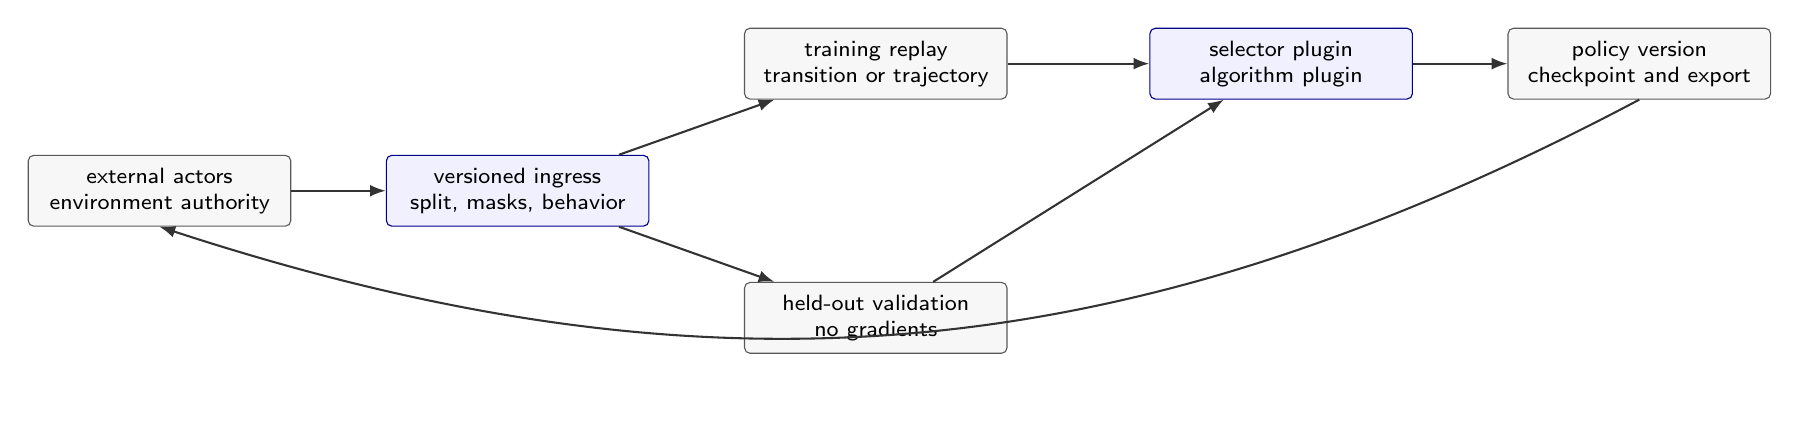
\begin{tikzpicture}[node distance=9mm and 12mm]
  \node[jbox] (actors) {external actors\\environment authority};
  \node[jhot,right=of actors] (ingress) {versioned ingress\\split, masks, behavior};
  \node[jbox,above right=7mm and 12mm of ingress] (train) {training replay\\transition or trajectory};
  \node[jbox,below right=7mm and 12mm of ingress] (valid) {held-out validation\\no gradients};
  \node[jhot,right=18mm of train] (learner) {selector plugin\\algorithm plugin};
  \node[jbox,right=of learner] (artifact) {policy version\\checkpoint and export};
  \draw[jflow] (actors) -- (ingress);
  \draw[jflow] (ingress) -- (train);
  \draw[jflow] (ingress) -- (valid);
  \draw[jflow] (train) -- (learner);
  \draw[jflow] (valid) -- (learner);
  \draw[jflow] (learner) -- (artifact);
  \draw[jflow,bend left=23] (artifact.south) to (actors.south);
\end{tikzpicture}
}%
\caption{The domain remains outside the learner.  Training and validation may
arrive interleaved, but routing precedes storage and creates two state-changing
contracts.}
\label{fig:system}
\end{figure}

Every public transition declares the split, actor, episode, timestep, and
policy version.  It contains current and next observations, chosen action,
reward, and terminal state.  Stochastic policy actors additionally retain the
behavior log probability and value estimate.  Boolean current and next legal
masks align with the model's declared action vocabulary.

The replay buffer stores action indices rather than domain objects.  A domain
action value can be supplied when it uniquely maps to one index.  This is a
bounded action contract: the compiler or application decides which slot means
close, wait, resize, hedge, or exercise, and the mask decides whether that slot
is admissible in the current state.

\subsection{Split isolation}

Training transitions update the running observation statistics and enter the
training replay.  Their priorities can change after an update.  Validation
transitions enter a separate bounded store.  They use the training
normalizer, but do not update it, change replay priority, execute optimizer
steps, or select a checkpoint implicitly.

The split is assigned before an episode begins.  Interleaving train and
validation items in one network request changes neither role.  For a pathwise
financial experiment, assigning individual steps from the same path to both
stores would still leak the path even though the service stores were separate;
scenario-level assignment therefore remains an actor responsibility.

\subsection{Trajectory construction}

Trajectory objectives require more than a bag of transitions.  The service
groups physical replay rows by actor and episode, orders them by timestep, and
splits a run at a missing timestep, terminal state, or configured rollout
length.  PPO, IMPALA, and APPO exclude fragments older than their configured
behavior-policy lag; offline MARWIL deliberately retains historical
demonstrations.  This produces actual contiguous traces for returns, GAE, or
V-trace rather than sorting an independently sampled batch after the fact.

Circular replay still means that an old prefix may have been overwritten.
The learner treats the surviving suffix as a fragment boundary.  It does not
invent continuity across missing rows.

\section{Plugin and artifact model}

\subsection{Algorithm contract}

An algorithm plugin has a semantic name and version, family, replay mode,
backend, default export module, description, noise profile, and agent factory.
The agent accepts arrays and plain metadata at the service boundary and
provides action selection, batched inference, training, held-out evaluation,
and state serialization.  Every update returns

\[
  U=(\ell,p_1,\ldots,p_B,\mathcal M),
\]

where $\ell$ is the update loss, $p_i$ is a replay-priority statistic
aligned with sampled row $i$, and $\mathcal M$ is an algorithm-specific
map of finite scalar metrics.  The runtime need not know whether $p_i$ came
from a TD error, a value loss, or another residual.

Built-ins register by importing their modules.  External packages use the
Python entry-point group \nolinkurl{jormungandr.algorithms}.  The selector has
an independent entry-point group,
\nolinkurl{jormungandr.rollout_selectors}.  One
broken optional package is isolated from built-ins during discovery.

\subsection{Checkpoint lifecycle}

The outer checkpoint remains \texttt{jormungandr.checkpoint.v1}.  Its payload
includes the resolved algorithm and plugin version, complete learner
configuration, policy and target tensors, optimizer states, observation
normalizer, feature order, action values, learner update, policy version,
selector identity, and model metadata.  Retaining the outer format preserves
the original C51 lifecycle while allowing a different state dictionary inside
it.  New plugin checkpoints refuse silent restore through a different plugin
name or version; a state-format change therefore requires an explicit
migration or a compatible semantic plugin version.

Replay and validation contents are not checkpointed.  A restored model resumes
parameters, optimizers, versions, and preprocessing but begins with empty
stores.  This distinction prevents a model checkpoint from being mistaken for
a complete distributed-job snapshot.

The exporter resolves the plugin's default Torch module and produces a
TorchScript file, JSON manifest, and generated C++ specification.  C51
manifests describe action-by-atom logits.  QR-DQN manifests describe
action-by-quantile values and retain the risk rule.  Policy and scalar-Q
profiles describe action-width outputs.  Torch checkpoints use pickle-based
loading and are therefore trusted local artifacts, not an untrusted
interchange format.

\section{Implemented algorithm profiles}

The service currently uses a fixed discrete action vocabulary for every
built-in.  Table~\ref{tab:algorithms} states the implemented profiles rather
than extending paper results to unimplemented observation or action spaces.

\begin{table}[H]
\centering
\scriptsize
\begin{tabularx}{\textwidth}{@{}P{0.13\textwidth}P{0.18\textwidth}X@{}}
\toprule
Plugin & Data mode & Implemented profile \\
\midrule
\texttt{c51} & off-policy & Categorical distributional Double-DQN on a fixed value support. \\
\texttt{qrdqn} & off-policy & Quantile-Huber Double QR-DQN with mean, lower-quantile, or CVaR action scoring. \\
\texttt{dqn} & off-policy & Double, dueling scalar Q-network with Huber TD loss. \\
\texttt{cql} & offline/off-policy & Discrete CQL(H) log-sum-exp penalty over the DQN objective. \\
\texttt{maxent} & off-policy & Discrete soft-Q Bellman backup and Boltzmann policy. \\
\texttt{bc} & demonstrations & Masked categorical behavior cloning. \\
\texttt{marwil} & offline trajectory & Moving-normalized, clipped exponential advantage weighting. \\
\texttt{ppo} & trajectory & GAE and clipped surrogate with multiple minibatch epochs. \\
\texttt{impala} & trajectory & V-trace actor--critic correction for behavior-policy lag. \\
\texttt{appo} & trajectory & IMPACT-style V-trace, target-policy clipping, and bounded circular replay. \\
\texttt{sac} & off-policy & Categorical SAC with twin critics, soft targets, and automatic temperature. \\
\texttt{dreamerv3} & model-based & Compact vector latent dynamics, symlog targets, imagination, and slow value target. \\
\bottomrule
\end{tabularx}
\caption{Built-in algorithm profiles.  The entries are service capabilities,
not claims of benchmark parity with every cited reference.}
\label{tab:algorithms}
\end{table}

\subsection{Value distributions}

C51 represents a return distribution with learned probabilities on fixed
support atoms \cite{c51}.  QR-DQN instead learns quantile locations
$\theta_i(s,a)$ at fixed fractions $\tau_i$ \cite{qrdqn}.  For target samples
$y_j$, its quantile-Huber loss is

\[
  \mathcal L=
  \frac{1}{N}\sum_{i=1}^{N}\sum_{j=1}^{N}
  \left|\tau_i-\mathbf 1\{y_j-\theta_i<0\}\right|
  L_\kappa(y_j-\theta_i).
\]

Expected-value control averages the learned quantiles.  A downside policy can
instead use the estimated lower quantile or average the lowest fraction as an
empirical lower-tail CVaR score.  These statistics expose aleatoric return
variation; they do not measure epistemic uncertainty and do not guarantee that
the tails are calibrated outside the data distribution.

DQN supplies the scalar baseline and uses Double-DQN selection to reduce
positive maximization bias \cite{dqn,doubleq}.  CQL adds a log-sum-exp conservative
penalty so unobserved actions are not assigned high values without a cost
\cite{cql}.  The implemented CQL profile is discrete; continuous CQL variants
are outside this service action contract.

\subsection{Policy, asynchronous, and offline objectives}

PPO clips the behavior-to-current policy ratio and uses generalized advantage
estimation \cite{ppo,gae}.  IMPALA applies V-trace corrections when actors and
the learner are decoupled \cite{impala}.  The APPO plugin follows the IMPACT
combination of a target policy, circular replay, and truncated importance
sampling rather than treating asynchronous PPO as ordinary shuffled replay
\cite{impact}.

Behavior cloning ignores reward and provides the demonstration baseline.
MARWIL estimates trajectory returns and a learned value, normalizes the
advantage scale with a moving statistic, and weights action likelihood by a
clipped exponential advantage \cite{marwil}.  CQL, BC, and MARWIL address
offline use in different ways; none licenses deployment outside the observed
state and action support without evaluation.

\subsection{Entropy and world models}

The maximum-entropy objective augments discounted reward with policy entropy,

\[
 J_\alpha(\pi)=\E_\pi\left[
   \sum_{t\geq0}\gamma^t
   \left(r(s_t,a_t)+\alpha\mathcal H(\pi(\cdot\mid s_t))\right)
 \right].
\]

The \texttt{maxent} plugin realizes this objective through discrete soft-Q
backups.  The SAC plugin uses a categorical actor, twin critics, soft target
updates, and optional automatic temperature \cite{sac}.  Illegal actions have
zero probability.  Their log probabilities are replaced only inside
expectations so the mathematical $0\log 0=0$ limit does not become an IEEE
NaN.

DreamerV3 learns a world model and improves an actor and critic through imagined
trajectories \cite{dreamerv3}.  The built-in profile retains vector encoding,
latent action dynamics, reward and continuation heads, symlog scaling,
imagination, lambda returns, and a slow value target.  It does not reproduce
the reference recurrent state-space model, categorical latent representation,
pixel decoder, or benchmark recipe.  Full DreamerV3 parity should be an
external plugin or a separately validated profile.

\section{Noise, disturbance, and risk}

\subsection{A disturbance taxonomy}

Reward outliers change the TD target; observation noise changes the estimated
state; stochastic transitions widen the return distribution; an offline
dataset changes support; actor lag changes the behavior policy; and a world
model introduces approximation bias.  One robustness label cannot distinguish
them.

The shared runtime offers training-only normalization, Huber losses in value
profiles, gradient clipping, optional reward clipping, and opt-in Gaussian
observation augmentation.  Reward clipping and augmentation are checkpointed
because they alter the objective.  A clean validation store remains clean by
default.  Named perturbed evaluation cohorts should carry the intended noise
law and severity.

Distributional critics are useful when outcome tails matter.  Double targets
and twin critics address value overestimation.  CQL addresses offline action
shift.  V-trace and APPO clipping address policy lag.  Dreamer transformations
address numerical scale, while held-out multi-step prediction must measure
world-model error.  Ensembles, adversarial observation training, explicit
robust-MDP optimization, and calibrated epistemic uncertainty are not
implemented merely by selecting one of these profiles.

\subsection{What maximum entropy proves}

Eysenbach and Levine show that maximum-entropy RL maximizes a lower bound on a
robust objective for characterized reward and transition disturbance sets
\cite{maxentrobust}.  The result supplies a principled hypothesis: an entropy
regularizer may retain multiple viable behaviors when one route or reward
perturbation changes.  It does not show that MaxEnt RL is optimal for every
sensor corruption, adversary, market regime, or reward misspecification.  The
temperature and disturbance family therefore belong in the experiment rather
than in a general robustness claim.

For noisy \VOLT{} outcomes, a predeclared comparison begins with DQN or PPO,
then compares QR-DQN under mean and fixed downside rules, and compares
categorical SAC or soft Q at fixed temperatures.  Seeds, path cohorts,
chronological dates, observation perturbations, and reward perturbations are
separate axes.  Choosing a CVaR level after inspecting held-out outcomes would
turn the held-out set into training data.

\section{QUBO rollout and frontier allocation}
\label{sec:qubo}

\subsection{The budgeted selection problem}

The computational problem is not to find a high-scoring path after every path
has been evaluated.  It is to decide which paths merit an expensive evaluation
using information that is already cheap.  Let $\mathcal{B}_{t-1}$ be the beam
retained at search depth $t-1$, and let

\[
 \mathcal{C}_t
 =\bigcup_{v\in\mathcal{B}_{t-1}}\operatorname{child}(v)
 =\{c_1,\ldots,c_{n_t}\}
\]

be the next candidate frontier.  Candidate $c_i$ has a cheap information set
$\mathcal{I}_{t,i}$---for example a policy/value estimate, an admissible bound,
a shallow rollout, or model disagreement---but an unknown expensive terminal
value $Y_i$.  A binary decision $x_i=1$ retains the candidate.  With a beam
budget $k_t$, the ideal one-step search decision is

\[
 \underset{x\in\{0,1\}^{n_t}}{\operatorname{arg\,max}}
 \quad
 \E\!\left[
   \max_{i:x_i=1}Y_i\,\middle|\,\mathcal{I}_t
 \right]
 \qquad
 \text{subject to}\qquad
 \mathbf{1}^{\mathsf T}x=k_t .
 \tag{1}
\]

The conditional joint distribution of the $Y_i$ is generally unavailable.
Moreover, selecting the individually largest point estimates can spend the
entire beam on highly correlated siblings whose errors share the same cause.
The implemented QUBO is therefore a tractable surrogate for (1): reward a
cheap utility estimate while charging for pairwise redundancy.  The recursion
is

\[
 \mathcal{B}_{t}=\{c_i\in\mathcal{C}_t:x_{t,i}=1\},
 \qquad \mathcal{B}_0=\{\text{root}\},
 \tag{2}
\]

and only $\mathcal{B}_D$ receives terminal evaluation at depth $D$.  The same
subset problem appears later in the learning pipeline when $c_i$ is a replay
transition or contiguous rollout fragment and $Y_i$ denotes unknown learning
value rather than terminal path value.  Search pruning is potentially more
valuable because it occurs before the expensive work.

Figure~\ref{fig:qubo-frontier-trace} makes the recursion explicit.  QUBO is
not applied independently inside each branch.  The retained parents are first
expanded, and one binary problem is formed over the complete frontier
$\mathcal{C}_t$.  Its single decision vector determines the next beam.

\begin{figure}[H]
  \centering
  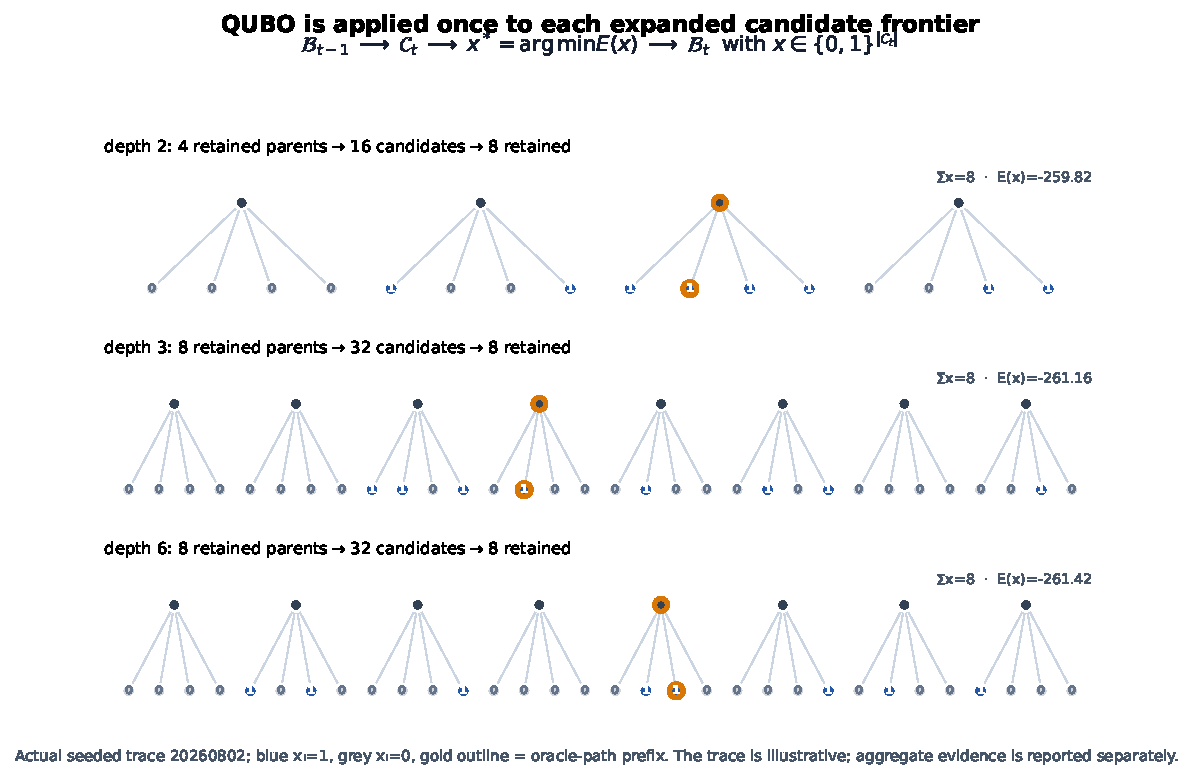
\includegraphics[width=\textwidth]{figures/qubo_frontier_trace.pdf}
  \caption{An actual width-eight trace for seed 20,260,802.  Blue nodes have
  $x_i=1$, grey nodes have $x_i=0$, and a gold outline identifies the
  oracle-path prefix known only to evaluation.  The trace explains the
  mechanism; the paired 500-tree experiment supplies aggregate evidence.}
  \label{fig:qubo-frontier-trace}
\end{figure}

\subsection{Utility and redundancy}

Let $\widehat v_i$ be the available scalar utility.  To prevent isolated
outliers from determining the linear QUBO coefficient, the implementation uses
the fifth and ninety-fifth percentiles $q_{.05}$ and $q_{.95}$:

\[
 u_i=\operatorname{clip}\!\left(
   \frac{\widehat v_i-q_{.05}}{q_{.95}-q_{.05}},0,1
 \right).
 \tag{3}
\]

If the percentile range is numerically zero, every candidate receives
$u_i=\tfrac12$.  Non-finite values are replaced by the finite median before
scaling.  In replay mode, the default unscaled utility is
$\widehat v_i=\operatorname{mean}_{j\in c_i}\log(1+p_j)$ for replay priority
$p_j$.  Absolute reward can be added but is disabled by default because it can
preferentially select lucky noisy outcomes.

Each candidate also has an embedding $z_i\in\mathbb{R}^{d}$.  For coordinate
$r$, define its median $m_r$, interquartile range $a_r$, and stabilized scale
$\bar a_r=a_r$ when $a_r>10^{-8}$ and $\bar a_r=1$ otherwise.  The robust
distance and RBF similarity are

\begin{equation}
\begin{aligned}
 \widetilde z_{ir} &= \frac{z_{ir}-m_r}{\bar a_r}, \\
 d_{ij}^{2} &= \lVert\widetilde z_i-\widetilde z_j\rVert_2^2, \\
 h &= \operatorname{median}\{d_{ij}^{2}:d_{ij}^{2}>10^{-12}\}, \\
 s_{ij} &= \exp\!\left(-\frac{d_{ij}^{2}}{2h}\right),
 \qquad s_{ii}=0 .
\end{aligned}
 \tag{4}
\end{equation}

The degenerate bandwidth is set to one.  Transition embeddings contain the
current state, state delta, action, reward, and terminal flag.  Rollout
embeddings summarize state and delta plus action, reward, terminal, and length.
In the path experiment below, a one-hot branch-position embedding makes paths
with long common prefixes similar.

\subsection{Constrained subset objective and QUBO matrix}

For $n$ candidates and target cardinality $k$, the binary energy is

\[
 E(x)=
 -\lambda_u\sum_{i=1}^{n}u_i x_i
 +\lambda_s\sum_{i<j}s_{ij}x_ix_j
 +\lambda_k\left(\sum_{i=1}^{n}x_i-k\right)^2,
 \qquad x_i\in\{0,1\}.
 \tag{5}
\]

The first term favors utility, the second charges for redundant pairs, and the
third turns the cardinality constraint into an unconstrained binary penalty.
Using $x_i^2=x_i$ and a symmetric convention $x^{\mathsf T}Qx$, expansion of
the final term gives

\[
 Q_{ii}=-\lambda_u u_i+\lambda_k(1-2k),
 \qquad
 Q_{ij}=\frac{\lambda_s s_{ij}+2\lambda_k}{2}\quad(i\ne j),
 \tag{6}
\]

such that $x^{\mathsf T}Qx=E(x)-\lambda_k k^2$.  The omitted constant cannot
change the minimizer.  Equation (6) is the exported Q matrix consumed by an
external annealer or binary optimizer.  An unconstrained backend must validate
that $\lambda_k$ is strong enough for its coefficient scale.  The built-in
solver instead stays in the feasible set $\mathbf{1}^{\mathsf T}x=k$, so its
cardinality is exact and the penalty is constant.

Within that feasible set, minimizing (5) is equivalent to maximizing

\[
 F(S)=\lambda_u\sum_{i\in S}u_i
      -\lambda_s\sum_{\substack{i<j\\i,j\in S}}s_{ij},
 \qquad |S|=k .
 \tag{7}
\]

The classical reference solver greedily adds the candidate with largest
marginal score

\[
 \Delta_i(S)=\lambda_u u_i-\lambda_s\sum_{j\in S}s_{ij},
 \tag{8}
\]

then applies deterministic one-for-one exchanges.  Replacing selected item
$o$ by unselected item $n$ changes (7) by

\[
 \Delta F_{o\rightarrow n}
 =\lambda_u(u_n-u_o)
 -\lambda_s\!\left(
   \sum_{j\in S\setminus\{o\}}s_{nj}
   -\sum_{j\in S\setminus\{o\}}s_{oj}
 \right).
 \tag{9}
\]

Positive exchanges are accepted until no one-swap improvement remains or the
configured pass limit is reached.  This is a classical local heuristic, not an
exact QUBO or quantum solver.  Q construction requires quadratic similarity
storage; the candidate-pool factor bounds $n$ in replay, and the beam bounds it
during search.  Candidate identities, decisions, energy, selected utility,
redundancy, matrix bytes, and solve time remain auditable.

The formulation follows QUBO episode selection \cite{quboepisodes};
quantum-inspired priority mechanisms provide a related replay direction
\cite{quantumreplay}.  They motivate the formulation but do not establish
quantum advantage.  Deterministic selection after prioritized sampling also
changes inclusion probabilities.  Ordinary PER weights do not correct this
second choice, so the implementation uses neutral learner weights and reports
the absence of an importance correction.

\subsection{Controlled branching experiment}

The empirical question is whether the diversity term can preserve a good
region under correlated heuristic error, and whether the saved evaluation
work can repay solve overhead.  Each of 500 paired trials constructs a complete
four-way tree of depth six.  A path is
$p=(a_1,\ldots,a_\ell)$ with $a_t\in\{0,1,2,3\}$.  Independent edge increments
at depth $t$ satisfy

\[
 \xi_{p_{1:t}}\sim\mathcal{N}(0,1/t),
 \qquad
 Y_p=\sum_{t=1}^{6}\xi_{p_{1:t}}
 \quad\text{for }|p|=6 .
 \tag{10}
\]

Thus the standard deviation of an increment is $1/\sqrt{t}$.  For every
prefix $p$, the benchmark oracle computes

\[
 M_p=\max_{q:\,p\text{ is a prefix of }q}Y_q .
 \tag{11}
\]

Search does not receive $M_p$ directly.  Its synthetic cheap estimate is

\[
 \widehat v_p=M_p+B_{a_1}+\varepsilon_p,
 \qquad
 B_a\sim\mathcal{N}(0,\sigma^2),
 \qquad
 \varepsilon_p\sim\mathcal{N}(0,(0.35\sigma)^2),
 \quad \sigma=0.9 .
 \tag{12}
\]

$B_{a_1}$ is shared by every path in a first-level region and therefore creates
the correlated optimism that diversity is intended to hedge;
$\varepsilon_p$ is independent.  The proxy is intentionally derived from the
oracle plus controlled noise.  It isolates subset selection and is not a claim
that a production value model knows subtree optima.

The tree contains $4^6=4{,}096$ terminal paths and
$\sum_{t=1}^{6}4^t=5{,}460$ non-root candidates.  Trial seeds are
$20{,}260{,}802+s$ for $s=0,\ldots,499$.  Utility-only search retains the top
$k$ values of $\widehat v$; monotone robust scaling does not change that order.
QUBO uses $\lambda_u=1$, $\lambda_s=0.12$, $\lambda_k=4$, and four local-swap
passes.  Beam widths $k\in\{4,6,8,10,12,16\}$ are evaluated on identical trees.

For terminal beam $\mathcal{B}_6$, oracle value $Y^*=M_{\emptyset}$, and
selected value $\widehat Y=\max_{p\in\mathcal{B}_6}Y_p$, the primary metrics are

\[
 R=Y^*-\widehat Y,
 \qquad
 H=\mathbf{1}\{R\le 10^{-12}\},
 \qquad
 G=\sum_{t=1}^{6}|\mathcal{C}_t|,
 \qquad
 L=|\mathcal{B}_6| .
 \tag{13}
\]

$R$ is simple terminal regret, $H$ is exact-optimum recovery, $G$ counts cheap
candidate generations, and $L$ counts terminal evaluations.  Mean-regret bars
use normal 95\% intervals; recovery bars use 95\% Wilson intervals.  Because
selectors see the same tree in each trial, paired regret improvement is
$D_s=R_{s,\mathrm{utility}}-R_{s,\mathrm{QUBO}}$ with interval

\[
 \overline D\ \pm\ 1.96\,s_D/\sqrt{500} .
 \tag{14}
\]

The run used one Python 3.11.15 process with NumPy 1.26 on an AMD Ryzen
Threadripper PRO 7985WX.  Timing is machine-specific; oracle construction is
evaluation instrumentation and is excluded from search accounting.

\begin{figure}[H]
  \centering
  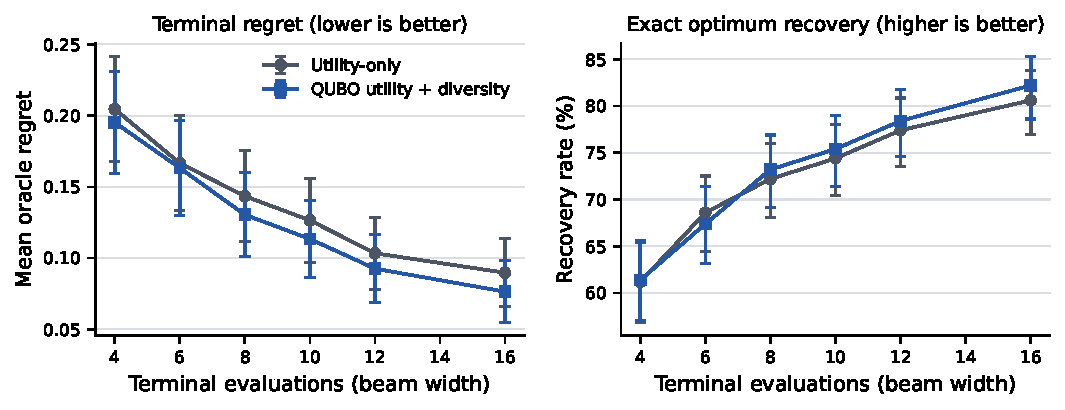
\includegraphics[width=\textwidth]{figures/qubo_frontier_efficiency.pdf}
  \caption{Paired frontier-search results over 500 trees.  QUBO has lower mean
  regret at every tested budget, but confidence intervals overlap at several
  widths; exact recovery is also slightly worse at width six.  Bars are the
  intervals defined after Equation~(13).}
  \label{fig:qubo-frontier-efficiency}
\end{figure}

\begin{table}[H]
\centering
\small
\caption{The two beam budgets used for the break-even comparison.}
\label{tab:qubo-frontier}
\begin{tabular}{llrrrrr}
\toprule
Selector & $k$ & Recovery & Mean $R$ & P95 $R$ & $G$ & Selector ms \\
\midrule
Utility & 8  & 72.2\% & 0.1435 & 1.0047 & 148 & 0.09 \\
QUBO    & 8  & 73.2\% & 0.1305 & 0.8060 & 148 & 2.87 \\
Utility & 10 & 74.4\% & 0.1266 & 0.7706 & 180 & 0.11 \\
QUBO    & 10 & 75.4\% & 0.1135 & 0.7230 & 180 & 3.57 \\
\bottomrule
\end{tabular}
\end{table}

At width eight, QUBO reduced mean regret from 0.1435 to 0.1305 and increased
exact recovery from 72.2\% to 73.2\%.  The paired mean improvement was
$\overline D=0.0130$ with 95\% interval $[0.0022,0.0239]$.  At width sixteen
the paired interval also excluded zero; at widths four, six, ten, and twelve
it did not.  At width six, QUBO reduced mean regret slightly but exact recovery
fell from 68.6\% to 67.4\%.  Figure~\ref{fig:qubo-frontier-efficiency} therefore
supports a bounded result: diversity improved average terminal quality in this
noise model, but did not dominate every metric at every budget.

\subsection{Compute break-even and interpretation}

Let $c_g$ be the average cost of generating and cheaply scoring one candidate,
$c_e$ the average terminal-evaluation cost, and $T_{s,A}$ selector time for
method $A$.  Its accounted search cost is

\[
 T_A=T_{s,A}+c_gG_A+c_eL_A .
 \tag{15}
\]

QUBO width eight is close in aggregate quality to utility width ten.  It uses
$G_Q=148$ rather than $G_U=180$ candidates and $L_Q=8$ rather than $L_U=10$
terminal evaluations.  It is faster whenever

\[
 32c_g+2c_e>T_{s,Q}-T_{s,U}\approx2.75\text{ ms} .
 \tag{16}
\]

If candidate generation is treated as free, Equation~(16) requires
$c_e>1.38$ ms per avoided terminal evaluation.  Any nonzero $c_g$ lowers that
threshold.  Conversely, if $\widehat v_i$ itself requires the full rollout,
the optimization is too late to recover rollout cost.

This experiment demonstrates a plausible classical QUBO integration benefit,
not an exact-solver, quantum, learning-performance, or Volt result.  It fixes
one synthetic error model and one coefficient set; it does not yet test
coefficient sensitivity, learned heuristic calibration, graph transpositions,
path-dependent market regimes, or end-to-end policy improvement.  The next
gate is a predeclared paired experiment on immutable Volt path cohorts using a
production-available cheap estimate and Equation~(15) for total wall time.

\section{Policy representation and Volt}

\subsection{Fixed embeddings and end-to-end encoders}

\VOLT{} constructs the option portfolio, state/action graph, action identity,
legal mask, financial transition, and reward evidence.  \JORM{} trains and
serves a statistical choice among the admissible action slots.  The boundary
does not grant the learner authority to create a contract, bypass a mask, or
apply a fill.

Deep Sets is the permutation-invariant set baseline \cite{deepsets}.  A typed
graph network adds relation-specific message passing when graph structure
earns its extra compute \cite{graphnet}.  A frozen encoder can produce a
fixed-size vector consumed by any service plugin today.  This is the simplest
path for entry selection, hold/close, and bounded hedge/resize stages.

The library also supplies an encoder-independent masked actor--critic loss.
Any Torch model that emits one policy-logit row and one value per state can use
it.  A graph trajectory buffer retains external state references, masks,
chosen slots, rewards, behavior probabilities, values, terminal flags, and
policy versions, then computes GAE targets.  A Volt in-process research driver
resolves references to Deep Sets or GNN batches and backpropagates through the
encoder.

The public service still stores fixed NumPy observations.  It does not define
a graph codec, batch variable numbers of nodes and actions through HTTP, or
checkpoint the graph artifact store.  Graph-native service training therefore
remains future work.  Hiding variable action semantics in an undocumented
fixed vector would make replay, masks, and checkpoints ambiguous.

\subsection{Quantile tree baselines}

CatBoost and LightGBM are useful after a Volt encoder has been frozen.  CatBoost
supports a multi-quantile objective in one CPU model; LightGBM supports a
quantile objective with an alpha parameter and normally uses one model per
level.  Both provide fast tree controls over numeric embeddings
\cite{catboost,lightgbm,catboostdocs,lightgbmdocs}.  Neither backpropagates through a Deep Sets or GNN
encoder.  Torch is therefore the default for end-to-end policy and critic
training.  Its distribution package supports categorical and reparameterized
sampling; QR-DQN itself requires only the differentiable quantile-Huber tensor
loss.

\section{Metrics and model comparison}

Every plugin reports common loss and priority statistics plus named internal
metrics such as entropy, value loss, Q mean, CQL penalty, temperature,
importance ratio, quantile spread, or model loss.  TensorBoard stores them
under algorithm-qualified paths.  The selector has a separate namespace.  A
runtime comparison endpoint aligns the latest rows for all model identifiers,
including externally logged held-out performance measures, and a per-model
endpoint retains recent history and the latest selection audit.

Objective losses from CQL, PPO, SAC, and Dreamer are not on one performance
scale.  Model selection uses predeclared held-out environment measures at equal
interaction or data budgets: return, lower-tail outcome, constraint events,
turnover, drawdown, stability across seeds, and inference/learner cost as the
domain requires.  Validation loss diagnoses its own objective; it does not by
itself choose the economically preferred policy.

\subsection{Controlled online transition comparison}

The first convergence experiment restricts its cohort to plugins that consume
the same online one-step transition stream: DQN, C51, QR-DQN, maximum-entropy
Soft-Q, and categorical SAC.  This is a compatibility condition, not a choice
of expected winners.  PPO, APPO, and IMPALA require behavior-policy
trajectories; BC, MARWIL, and CQL require a declared offline dataset; and
DreamerV3 needs a sequence and model-compute budget.  Putting those objectives
on this curve would change both their input data and their update budget.

Each included algorithm uses a two-layer width-64 network, learning rate
$3\times10^{-4}$, discount $0.97$, prioritized replay, batch size 32, and its
native exploration rule.  Five independently initialized runs receive 64
fixed-schedule episodes of the synthetic OU spread environment, each of length
32.  Replay warms for 128 transitions, after which one update follows every
new transition, giving 2,048 interactions and 1,921 updates per run.  Every
four episodes the deterministic policy is evaluated without learning on the
same 16 held-out path seeds.  A second cohort adds independent
$\mathcal{N}(0,0.15^2)$ noise to the spread and spread-change sensors while
leaving position and remaining time exact.  Intervals are
$\overline R\pm1.96s_R/\sqrt{5}$ across the five run-level held-out means.

\begin{figure}[H]
  \centering
  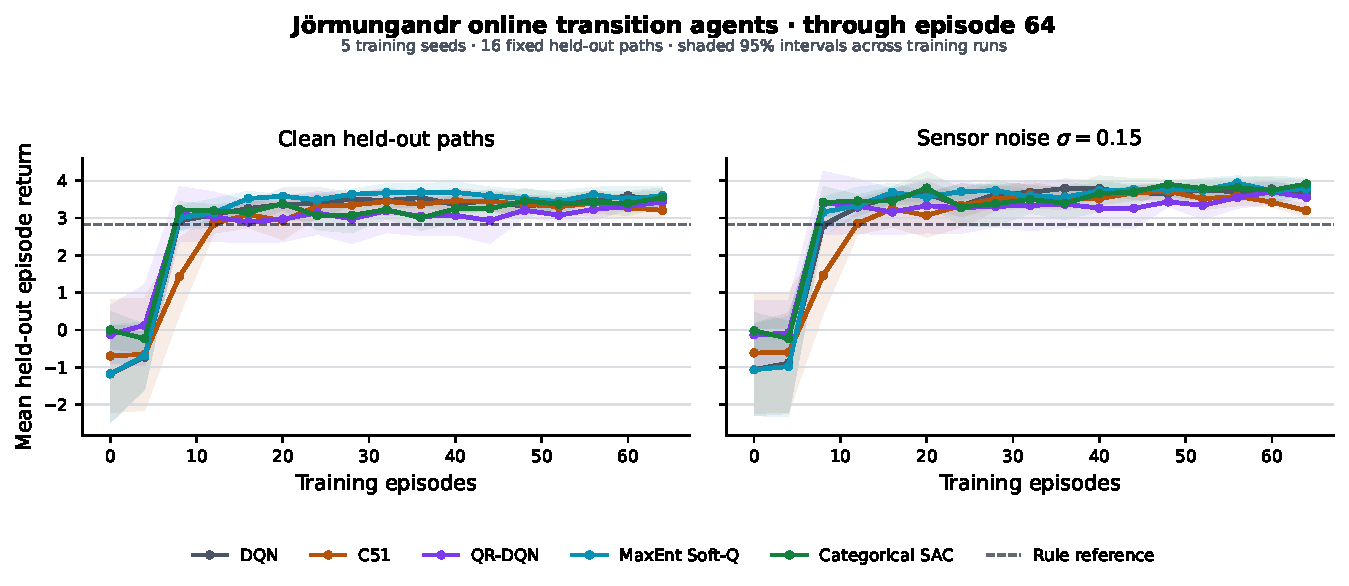
\includegraphics[width=\textwidth]{figures/ou_algorithm_convergence.pdf}
  \caption{Held-out convergence for compatible online transition learners.
  The dashed rule reference returns 2.8367 on the fixed paths.  Shading is the
  normal 95\% interval across five independent training runs; it describes
  training-seed variation on this cohort, not environment-general uncertainty.}
  \label{fig:ou-algorithm-convergence}
\end{figure}

\begin{table}[H]
\centering
\small
\caption{Final mean held-out episode return with normal 95\% intervals.}
\label{tab:ou-algorithm-convergence}
\begin{tabular}{lcc}
\toprule
Algorithm & Clean & Sensor noise $\sigma=0.15$ \\
\midrule
DQN             & 3.4413 $[3.1439,3.7387]$ & 3.6837 $[3.5181,3.8493]$ \\
C51             & 3.2101 $[3.0546,3.3655]$ & 3.1983 $[3.0047,3.3919]$ \\
QR-DQN          & 3.4382 $[3.1950,3.6814]$ & 3.5558 $[3.3141,3.7974]$ \\
MaxEnt Soft-Q   & 3.6087 $[3.3839,3.8334]$ & 3.7893 $[3.5476,4.0310]$ \\
Categorical SAC & 3.5508 $[3.2913,3.8104]$ & 3.9155 $[3.7581,4.0728]$ \\
\bottomrule
\end{tabular}
\end{table}

Most agents crossed the reference point estimate at the episode-eight
checkpoint; C51 improved more slowly.  MaxEnt Soft-Q has the largest final
clean point estimate and SAC the largest perturbed point estimate, but their
intervals overlap several alternatives.  Perturbation also improves some
point estimates in this threshold-like environment.  The result therefore
demonstrates a functioning comparison protocol and exposes behavioral
differences; it does not establish a general winner or a robustness guarantee.
The committed animation reveals convergence checkpoints, and a separate
same-path playback shows final median-run actions and accumulated reward.  The
single playback path is explanatory rather than additional evidence.

\section{Python, Torch, and a future Rust path}

Python is appropriate for orchestration and research iteration, while Torch
owns modules, automatic differentiation, device execution, and model export.
The first native migration should follow profiles rather than intuition.  The
likely CPU candidates are replay indexing, contiguous-fragment assembly, QUBO
construction and local search, graph collation, preprocessing, and return
kernels such as GAE or V-trace.

A PyO3 extension can preserve the plugin boundary by accepting contiguous
arrays and returning priorities, metrics, selections, or tensors.  DLPack or a
documented NumPy ownership contract avoids copies.  Keeping policy modules in
Torch avoids a second optimizer and checkpoint ecosystem.  A native backend
must retain semantic plugin version, tensor names or an explicit migration,
dtype and shape contracts, deterministic seeds, and parity tests against the
Python reference.

Moving the whole algorithm to Rust before measurement would enlarge the
artifact and autograd boundary.  Moving a quadratic selector or replay scan
after it dominates a profile is a smaller and testable change.  The current
plugin metadata already records \texttt{python-torch}; a future backend can
declare \texttt{rust-pyo3-torch} without changing actor messages.

\section{Current implementation and limits}

The public implementation registers twelve profiles: C51, QR-DQN, DQN, CQL,
maximum-entropy soft Q, BC, MARWIL, PPO, IMPALA, APPO, categorical SAC, and the
compact DreamerV3 profile.  The HTTP service lists plugins, applies legal masks
at inference and backup, stores behavior metadata, assembles contiguous
trajectories, filters excessive policy lag for online trajectory learners,
selects ordinary or QUBO batches, logs algorithm-qualified metrics,
checkpoints arbitrary plugin state, restores it, and exports each plugin's
declared Torch module.

The recorded functional suite contains 48 passing cases.  It includes direct
finite updates and state round trips for every built-in, C51 projection and
mask checks, graph-reference GAE, validation isolation, HTTP ingress, masked
SAC entropy, QR-DQN tail output, QUBO cardinality and fragment audit, checkpoint
restore, frontier accounting and local-swap checks, replayable visualization
audits, the seeded online comparison harness, and artifact manifests.  A
separate threaded matrix gave every built-in eight mask-aware transitions;
each completed an update, checkpoint, TorchScript export, restore, and masked
inference.

These are lifecycle tests.  They do not reproduce Atari, continuous-control,
Minecraft, offline-RL, or Volt trading benchmarks.  The built-in CQL and SAC
profiles are discrete.  The Dreamer profile is smaller than the reference.
Replay data are not durable across restart.  Graph-native HTTP transport,
dynamic action descriptors, multi-learner synchronization, authentication,
binary high-throughput transport, exact QUBO solving, native kernels, and a
Volt-scale empirical QUBO advantage remain outside the release.

\section{Conclusion}

An RL library should preserve experiment identity while allowing the learning
rule to change.  \JORM{} keeps actors, splits, masks, replay provenance,
versions, validation, metrics, and artifacts stable, and makes algorithms and
rollout allocation replaceable plugins.  Distributional, offline,
asynchronous, maximum-entropy, and model-based profiles can therefore be
compared through one lifecycle without calling the system a C51 model.

Quantile regression supplies a direct return-risk representation for noisy
outcomes; maximum entropy supplies a bounded robustness hypothesis; CQL and
V-trace address different shifts.  QUBO supplies an auditable allocation
experiment whose binary unit is a rollout fragment or frontier node.  Volt
retains financial and graph authority while Torch set or graph models supply the policy.  Rust
can later accelerate measured CPU kernels behind the same contracts.  The
remaining test is empirical: under predeclared disturbances, paths, budgets,
and controls, do these results survive valid offline, trajectory, model-based,
and Volt-scale cohorts, and does added complexity repay its compute cost?

\begin{thebibliography}{99}

\bibitem{dqn}
V. Mnih et al.,
\emph{Human-level control through deep reinforcement learning},
Nature 518, pp.~529--533, 2015,
\url{https://doi.org/10.1038/nature14236}.

\bibitem{doubleq}
H. van Hasselt, A. Guez, and D. Silver,
\emph{Deep Reinforcement Learning with Double Q-learning},
AAAI Conference on Artificial Intelligence, 2016,
\url{https://arxiv.org/abs/1509.06461}.

\bibitem{c51}
M. G. Bellemare, W. Dabney, and R. Munos,
\emph{A Distributional Perspective on Reinforcement Learning},
International Conference on Machine Learning, 2017,
\url{https://arxiv.org/abs/1707.06887}.

\bibitem{qrdqn}
W. Dabney, M. Rowland, M. G. Bellemare, and R. Munos,
\emph{Distributional Reinforcement Learning with Quantile Regression},
AAAI Conference on Artificial Intelligence, 2018,
\url{https://arxiv.org/abs/1710.10044}.

\bibitem{per}
T. Schaul, J. Quan, I. Antonoglou, and D. Silver,
\emph{Prioritized Experience Replay},
International Conference on Learning Representations, 2016,
\url{https://arxiv.org/abs/1511.05952}.

\bibitem{gae}
J. Schulman, P. Moritz, S. Levine, M. Jordan, and P. Abbeel,
\emph{High-Dimensional Continuous Control Using Generalized Advantage
Estimation},
International Conference on Learning Representations, 2016,
\url{https://arxiv.org/abs/1506.02438}.

\bibitem{ppo}
J. Schulman, F. Wolski, P. Dhariwal, A. Radford, and O. Klimov,
\emph{Proximal Policy Optimization Algorithms}, 2017,
\url{https://arxiv.org/abs/1707.06347}.

\bibitem{impala}
L. Espeholt et al.,
\emph{IMPALA: Scalable Distributed Deep-RL with Importance Weighted
Actor-Learner Architectures},
International Conference on Machine Learning, 2018,
\url{https://arxiv.org/abs/1802.01561}.

\bibitem{impact}
M. Luo, J. Yao, R. Liaw, E. Liang, and I. Stoica,
\emph{IMPACT: Importance Weighted Asynchronous Architectures with Clipped
Target Networks},
International Conference on Learning Representations, 2020,
\url{https://arxiv.org/abs/1912.00167}.

\bibitem{sac}
T. Haarnoja, A. Zhou, P. Abbeel, and S. Levine,
\emph{Soft Actor-Critic: Off-Policy Maximum Entropy Deep Reinforcement
Learning with a Stochastic Actor},
International Conference on Machine Learning, 2018,
\url{https://arxiv.org/abs/1801.01290}.

\bibitem{cql}
A. Kumar, A. Zhou, G. Tucker, and S. Levine,
\emph{Conservative Q-Learning for Offline Reinforcement Learning},
Advances in Neural Information Processing Systems, 2020,
\url{https://arxiv.org/abs/2006.04779}.

\bibitem{marwil}
Q. Wang, J. Xiong, L. Han, P. Sun, H. Liu, and T. Zhang,
\emph{Exponentially Weighted Imitation Learning for Batched Historical Data},
Advances in Neural Information Processing Systems, 2018,
\url{https://proceedings.neurips.cc/paper/2018/hash/4aec1b3435c52abbdf8334ea0e7141e0-Abstract.html}.

\bibitem{dreamerv3}
D. Hafner, J. Pasukonis, J. Ba, and T. Lillicrap,
\emph{Mastering Diverse Domains through World Models}, 2023,
\url{https://arxiv.org/abs/2301.04104}.

\bibitem{maxentrobust}
B. Eysenbach and S. Levine,
\emph{Maximum Entropy RL (Provably) Solves Some Robust RL Problems},
International Conference on Learning Representations, 2022,
\url{https://arxiv.org/abs/2103.06257}.

\bibitem{deepsets}
M. Zaheer, S. Kottur, S. Ravanbakhsh, B. P\'oczos, R. Salakhutdinov, and
A. Smola,
\emph{Deep Sets},
Advances in Neural Information Processing Systems, 2017,
\url{https://arxiv.org/abs/1703.06114}.

\bibitem{graphnet}
P. W. Battaglia et al.,
\emph{Relational Inductive Biases, Deep Learning, and Graph Networks}, 2018,
\url{https://arxiv.org/abs/1806.01261}.

\bibitem{quboepisodes}
H. Salloum, A. Jnadi, Y. Kholodov, and A. Gasnikov,
\emph{Quantum-Inspired Episode Selection for Monte Carlo Reinforcement
Learning via QUBO Optimization}, 2026,
\url{https://arxiv.org/abs/2601.17570}.

\bibitem{quantumreplay}
C. Y. Chen, H. H. Hsu, and H. T. Lin,
\emph{Quantum-Inspired Experience Replay}, 2021,
\url{https://arxiv.org/abs/2101.02034}.

\bibitem{catboost}
L. Prokhorenkova, G. Gusev, A. Vorobev, A. Dorogush, and A. Gulin,
\emph{CatBoost: Unbiased Boosting with Categorical Features},
Advances in Neural Information Processing Systems, 2018,
\url{https://arxiv.org/abs/1706.09516}.

\bibitem{lightgbm}
G. Ke et al.,
\emph{LightGBM: A Highly Efficient Gradient Boosting Decision Tree},
Advances in Neural Information Processing Systems, 2017,
\url{https://proceedings.neurips.cc/paper/2017/hash/6449f44a102fde848669bdd9eb6b76fa-Abstract.html}.

\bibitem{catboostdocs}
CatBoost,
\emph{Regression objectives},
\url{https://catboost.ai/docs/en/concepts/loss-functions-regression}.

\bibitem{lightgbmdocs}
LightGBM,
\emph{Parameters},
\url{https://lightgbm.readthedocs.io/en/stable/Parameters.html}.

\end{thebibliography}

\end{document}
